\section{Experimental Results}
\ifCLASSOPTIONonecolumn\begin{figure*}[t]
\centering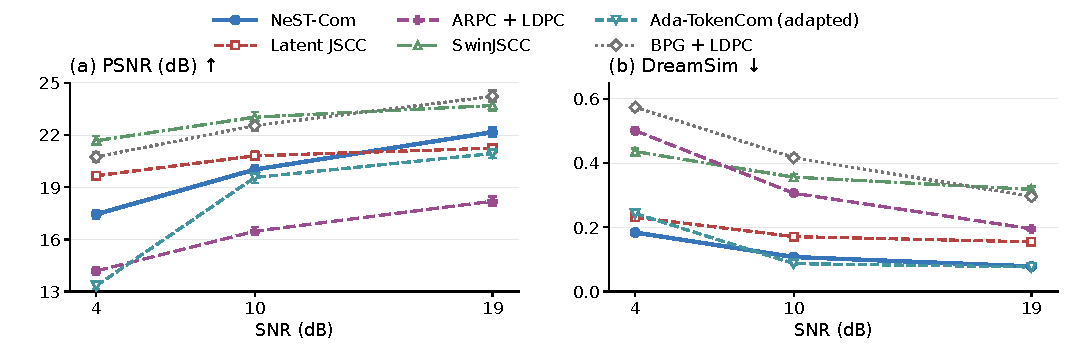
\includegraphics[width=\textwidth]{figure2.pdf}
\caption{Performance on 500 ImageNet validation images at $N=1024$. Error bars show 95\% source-bootstrap confidence intervals. Ada denotes the fixed-frame adaptation.}
\label{fig:performance}
\end{figure*}
\fi
\subsection{Experimental Setup}
We use common500 ImageNet validation images~\cite{imagenet}, a disjoint cal1000 set, and Kodak24~\cite{kodak}, with fixed $256\times256$ preprocessing. ImageNet-calibrated policies remain fixed on Kodak. The six-system main study uses $N=1024$; NeST, WHOLE, and Ada also use $N=512$, each independently calibrated at 4/10/19~dB.

Our convolutional Latent JSCC maps tokenizer latents to symbols and shares $\Dc$, using MSE, LPIPS, and latent-consistency losses. It and SwinJSCC~\cite{swinjscc}, adapted to $256\times256$ and $N=1024$, use the same 20\,000 training images and final 100k/200k-update checkpoints. Digital baselines are adaptive BPG~\cite{bpg} + LDPC, ARPC~\cite{arpc} + LDPC with paid captions, and Ada-TokenCom~\cite{adatokencom} adapted to the same fixed single-frame budget. Ada retains LlamaGen-L/VQ16 and prefix arithmetic coding, with a fixed ConvNeXt predicting a paid 10-bit class. Its sampled tail uses CFG=4, $T=1$, top-$k=2000$, and top-$p=1$. Full configurations and training records accompany this letter.

Metrics are PSNR, LPIPS-Alex~\cite{lpips}, DreamSim~\cite{dreamsim}, and CLIP ViT-L/14 image--image cosine (CLIP-I)~\cite{clip}. Frozen FP32 preprocessing uses $224\times224$ bicubic-antialias inputs for DreamSim/CLIP. Three channel outcomes per image, including the gray outputs defined in Sec.~II-C, are averaged before equal-source means and direct source-paired 95\% bootstrap intervals (10\,000 resamples). Endpoint, receiver, and decoding controls use a fixed 100-image subset. Complete four-metric diagnostics and statistical identities are provided in the supplementary material.

\ifCLASSOPTIONonecolumn\else\begin{figure*}[t]
\centering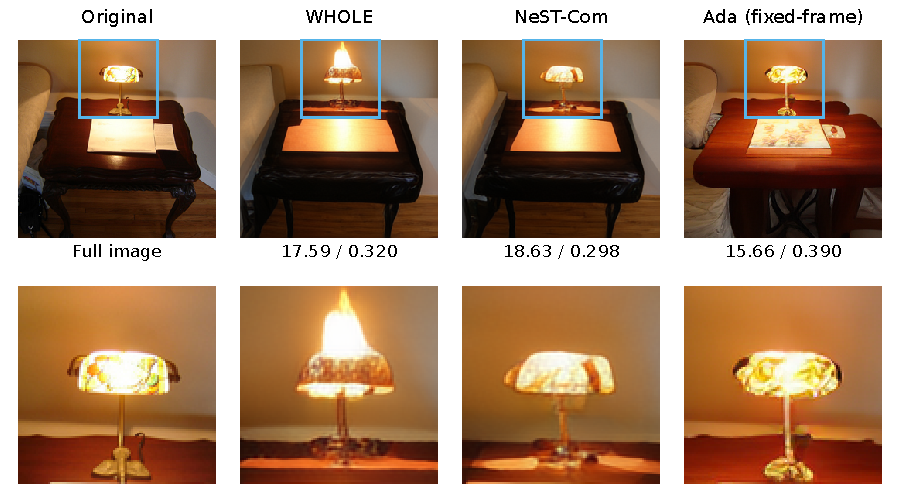
\includegraphics[width=6.0in]{figure3.pdf}
\caption{Example reconstructions at $N=512$ and 10~dB. The top row shows full images and the bottom row enlarges the same marked region. Values denote full-image PSNR$\uparrow$ / LPIPS$\downarrow$. Ada denotes the fixed-frame adaptation.}
\label{fig:qualitative}
\end{figure*}
\fi
\subsection{Effect of Within-Scale Endpoints}
\begin{table}[t]
\caption{Within-scale endpoint and receiver evidence. (A) Main family-specific policies; differences are PARTIAL minus WHOLE. (B) Controlled granularity on 100 sources with fixed model, MCS, maximum endpoint and fitting rule. (C) Receiver interventions on the same 100 sources and actual prefixes. Brackets give source-paired 95\% CIs; populations and conditions are as stated.}
\label{tab:internal}
\centering\footnotesize
\setlength{\tabcolsep}{2.5pt}
\begin{tabular}{ccc}
\toprule
\multicolumn{3}{l}{(A) Main policies at $N=1024$} \\
SNR & Util. W$\to$P (\%) & $\Delta$PSNR (dB) [95\% CI] \\
\midrule
\multicolumn{3}{l}{common500} \\
4 & 73.81 $\to$ 93.08 & $+0.616\;[0.564,0.673]$ \\
10 & 77.70 $\to$ 95.21 & $+0.701\;[0.637,0.766]$ \\
19 & 85.24 $\to$ 94.73 & $+0.319\;[0.290,0.349]$ \\
\multicolumn{3}{l}{Kodak24} \\
4 & 75.69 $\to$ 93.43 & $+0.396\;[0.236,0.543]$ \\
10 & 78.11 $\to$ 94.99 & $+0.674\;[0.408,0.958]$ \\
19 & 85.69 $\to$ 93.71 & $+0.228\;[0.140,0.324]$ \\
\midrule
\multicolumn{3}{l}{(B) Fixed-granularity diagnostic, 10 dB} \\
Grid (candidates) & Utilization (\%) & PSNR (dB) \\
Whole (7) & 78.15 & 18.952 \\
Half (13) & 89.21 & 19.396 \\
Quarter (25) & 95.38 & 19.612 \\
Eighth (49) & 97.39 & 19.735 \\
\midrule
\multicolumn{3}{l}{(C) Receiver interventions: $\Delta$PSNR (dB) [95\% CI]} \\
SNR & B0$-$A0 & C0$-$B0 \\
10 & $+0.220\;[0.176,0.264]$ & $+0.440\;[0.330,0.558]$ \\
19 & $+0.301\;[0.247,0.358]$ & $+0.000\;[0.000,0.000]$ \\
\bottomrule
\end{tabular}
\end{table}

Table~\ref{tab:internal}(A) compares WHOLE/PARTIAL with shared tokenizer, prior, entropy coder, and $\Dc$. Separate family calibration selects the same MCS at each SNR. Common500 PSNR gains are 0.616/0.701/0.319~dB at 4/10/19~dB. At 10~dB, source-bit utilization rises from 77.70\% to 95.21\% and DreamSim falls by 0.0240. On Kodak, the corresponding PSNR gain is 0.674~dB and DreamSim decreases by 0.0164; its 19~dB DreamSim interval includes zero. The higher utilization retains additional source tokens within the same frame.

Block~B fixes the 100 sources, model, MCS, maximum endpoint, and fitting rule. Whole/Half/Quarter/Eighth grids increase utilization from 78.15\% through 89.21\% and 95.38\% to 97.39\%, with PSNR increasing from 18.952 to 19.735~dB. Relative to the predefined Quarter configuration, Eighth adds $0.123\,[0.079,0.169]$~dB at 10~dB; its DreamSim/CLIP-I difference intervals cross zero.

Block~C uses the same 100 sources and actual received prefixes. A0 ignores received boundary tokens and follows the prior. B0 adds their correction to the final residual latent while finer-scale conditioning follows A0. C0 updates both latent and conditioning. The ordered PSNR gains are 0.220 and 0.440~dB at 10~dB, supporting both uses of received boundary tokens. At 19~dB, the boundary lies in the last scale, so the additional conditioning update has zero effect.

\emph{Completion versus coarse decoding:} With an identical received WHOLE prefix and the same adapted decoder, next-scale completion reduces DreamSim by 0.420 and 0.452 at $N=512$, 4 and 10~dB, respectively. Its PSNR changes are $+0.026\,[-0.204,0.271]$ and $+0.771\,[0.563,0.986]$~dB on the fixed 100-image subset. LPIPS decreases and CLIP-I increases at both points with paired intervals excluding zero. Completion improves these perceptual measures at both operating points, with a clear PSNR benefit at 10~dB.

\subsection{Comparison With Existing Methods}
\begin{table}[t]
\caption{Perceptual distance and image-feature similarity on common500 at $N=1024$. Each cell is LPIPS-Alex$\downarrow$ / CLIP-I$\uparrow$. Ada denotes the fixed-frame adaptation. Values are source means.}
\label{tab:external}
\centering\footnotesize
\setlength{\tabcolsep}{3pt}
\begin{tabular}{lccc}
\toprule Method & 4 dB & 10 dB & 19 dB \\
\midrule
NeST-Com & 0.263 / 0.821 & 0.171 / 0.873 & 0.118 / 0.900 \\
Latent JSCC & 0.219 / 0.741 & 0.173 / 0.789 & 0.158 / 0.804 \\
SwinJSCC & 0.530 / 0.627 & 0.469 / 0.669 & 0.440 / 0.697 \\
BPG + LDPC & 0.725 / 0.586 & 0.589 / 0.635 & 0.458 / 0.684 \\
ARPC + LDPC & 0.512 / 0.644 & 0.341 / 0.713 & 0.250 / 0.788 \\
Ada (adapted) & 0.395 / 0.828 & 0.167 / 0.884 & 0.138 / 0.892 \\
\bottomrule
\end{tabular}
\end{table}

Fig.~\ref{fig:performance} and Table~\ref{tab:external} show the complete-system tradeoffs at $N=1024$. NeST exceeds Ada in PSNR by 4.116/0.455/1.226~dB at 4/10/19~dB and exceeds ARPC by 3.26--3.97~dB. Ada has better LPIPS, DreamSim, and CLIP-I at 10~dB, higher CLIP-I at 4~dB, and slightly lower DreamSim at 19~dB. SwinJSCC and BPG have higher PSNR than NeST throughout; Latent JSCC has higher PSNR at 4/10~dB and lower LPIPS at 4~dB. Thus the source-constrained generative route offers a different balance between pixel fidelity and perceptual reconstruction.

\subsection{Transmission With a Reduced Symbol Budget}
\ifCLASSOPTIONonecolumn\begin{figure*}[t]
\centering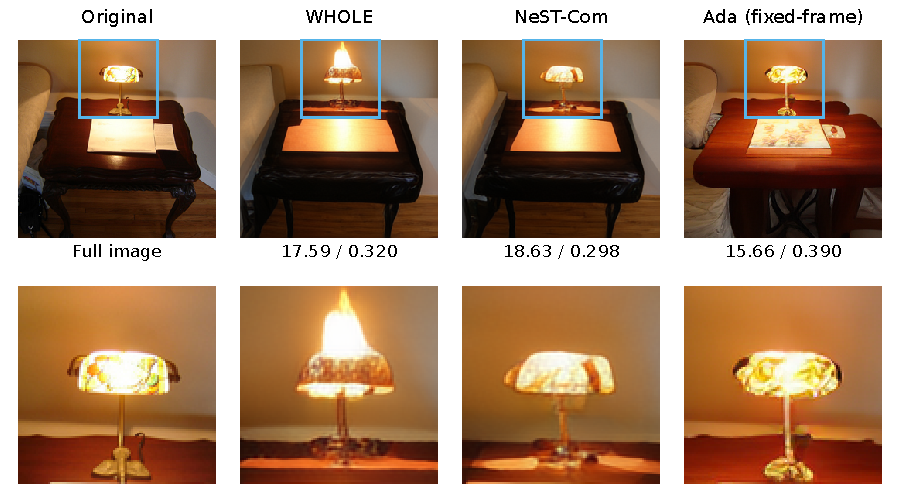
\includegraphics[width=6.0in]{figure3.pdf}
\caption{Example reconstructions at $N=512$ and 10~dB. The top row shows full images and the bottom row enlarges the same marked region. Values denote full-image PSNR$\uparrow$ / LPIPS$\downarrow$. Ada denotes the fixed-frame adaptation.}
\label{fig:qualitative}
\end{figure*}
\fi
\begin{table}[t]
\caption{Reduced-budget comparison on common500 at $N=512$. Differences are NeST-Com minus the fixed-frame Ada-TokenCom adaptation; brackets give source-paired 95\% CIs. Positive PSNR and negative DreamSim favor NeST-Com.}
\label{tab:reduced}
\centering\footnotesize
\setlength{\tabcolsep}{4pt}
\begin{tabular}{ccc}
\toprule SNR & $\Delta$PSNR (dB) & $\Delta$DreamSim \\
\midrule
4 & $+4.180$ & $-0.1029$ \\
 & $[3.991,4.377]$ & $[-0.1142,-0.0917]$ \\
10 & $+4.055$ & $-0.0660$ \\
 & $[3.880,4.235]$ & $[-0.0747,-0.0573]$ \\
19 & $+1.740$ & $+0.0139$ \\
 & $[1.577,1.909]$ & $[0.0103,0.0173]$ \\
\bottomrule
\end{tabular}
\end{table}

At $N=512$, 68 header symbols leave 444 body symbols. NeST improves over WHOLE by $0.392\,[0.341,0.444]$, $0.399\,[0.356,0.445]$, and $0.792\,[0.740,0.844]$~dB at 4/10/19~dB. All corresponding LPIPS, DreamSim, and CLIP-I paired intervals also favor NeST. At 10~dB, WHOLE and NeST select the same target $(7,0)$ and 16-QAM rate-2/3 MCS. When that target exceeds an image's capacity, within-scale fallback endpoints preserve more of its description than the preceding whole scale, raising utilization from 79.30\% to 93.46\%.

WHOLE already has higher mean PSNR than Ada by 3.79/3.66/0.95~dB. NeST increases these gaps to 4.180/4.055/1.740~dB (Table~\ref{tab:reduced}) and has lower LPIPS at all three SNRs. DreamSim favors NeST at 4/10~dB and Ada at 19~dB; CLIP-I favors Ada throughout. Fig.~\ref{fig:qualitative} shows how the additional within-scale tokens improve the reconstructed lamp-shade geometry relative to whole-scale transmission.

On the fixed 100-image subset, replacing Ada's sampled tail with greedy decoding preserves NeST-Com's low-budget PSNR advantage, yielding gains of 4.63 and 4.60~dB at 4 and 10~dB, respectively. The original sampling baseline remains the main comparison; complete sensitivity results, including $N=1024$, are in the supplement.
